%% figure 객체: fig:kill-gap-kde — 잇따른 킬 사이 간격의 커널 밀도와 시간 경계.
%% 원본 figures/kill_gap_kde.png. 저장소의 잠긴 경계 기록에서 곡선을 되살려 그린 것이며,
%% 되살린 봉우리·골·깊이가 기록값과 일치함이 확인되어 있다 (lock_match).
\begin{figure}[t]
  \centering
  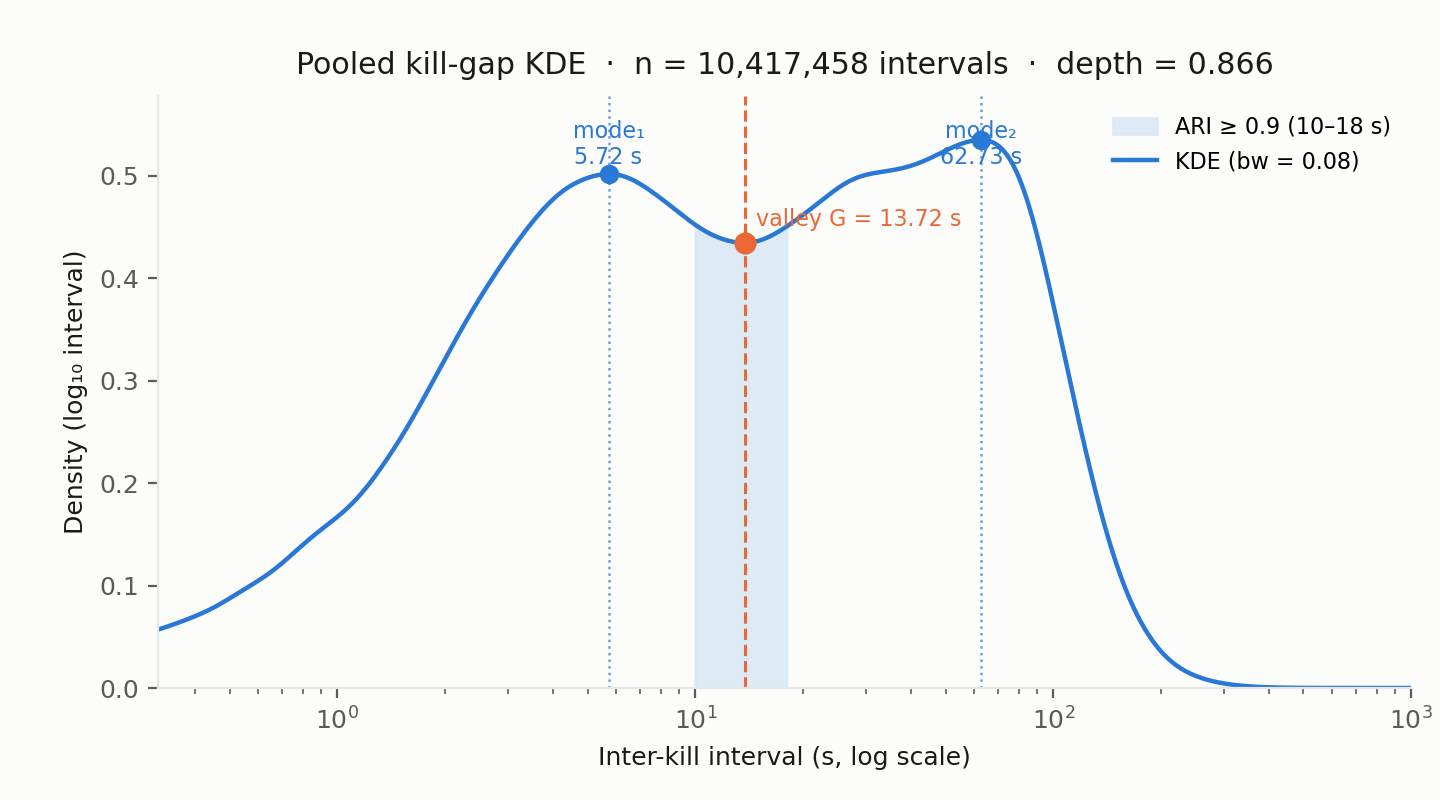
\includegraphics[width=\linewidth]{figures/kill_gap_kde.png}
  \caption{잇따른 킬 사이 간격의 분포와 시간 경계}
  \label{fig:kill-gap-kde}
\end{figure}
